\subsection{Glyph: \glyph{Unknown influence}}
\label{sec:af:unknown_infl}

An \emph{unknown influence} is used when the effect exerted from one activity to another is not well understood, or sometimes understood but complex.

\begin{glyphDescription}

\glyphSboTerm SBO:0000168 ! control

 \glyphOrigin Any \glyph{biological activity} (\sect{af:biologicalActivity}) or any \glyph{logical operator} (\sect{af:logic}).
 \glyphTarget Any \glyph{biological activity} (\sect{af:biologicalActivity}) or \glyph{phenotype} (\sect{af:phenotype}).
 \glyphEndPoint The target extremity of a \glyph{unknown influence} carries an open diamond (\fig{af:unknownInfl}).

\end{glyphDescription}

\begin{figure}[H]
  \centering
  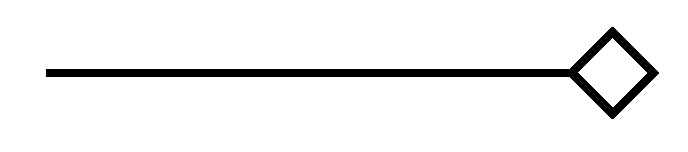
\includegraphics[width = 2in]{images/build/unknownInfluence.pdf}
  \caption{The \AF glyph for \glyph{unknown influence}.}
  \label{fig:af:unknownInfl}
\end{figure}

